\chapter{Concept}
\label{ch:concept}

\section{Présentation}
\label{sec:concept_introduction}

Un VESAD est une technique d'aggrandissement d'un écran physique par RA : un visiocasque de RA affiche un écran virtuel placé automatiquement autour d'écran physique que l'on souhaite étendre, sur le même plan que lui ; les deux écrans étant synchronisés, l'utilisateur peut alors voir et interagir avec comme s'il s'aggissait d'un seul écran étendu. Cette technique peut ainsi être appliquée pour tout type d'écran, incluant ceux des ordinateurs, les télévisions ou les affichages muraux. Nous travaillons cependant seulement avec l'aggrandissement de l'écran d'un téléphone intelligent dans ce mémoire. Notre premier sous-problème est de concevoir l'IHM d'un VESAD sur un téléphone : nous décrivons donc quelques applications et techniques d'interactions potentielles de ce concept.

Notre concept est d'une certaine manière un cas particulier du Personal Cockpit : une seule fenêtre, étendue, située sur le téléphone. On peut très bien imaginer une coexistence des deux designs : des fenêtres autour de soi, dans des espaces de travail (comme le propose hololens), et d'autres liées à notre téléphone qu'on peut porter avec soi.

Notre concept est également dans la continuité de la condition \condition{Smartwatch referenced} de MultiFi \citep{Grubert2015} où une montre intelligente est étendue par un visiocasque de RA.

Enfin, nous situons notre concept par rapport au cadre de conception proposé par \cite{Ens2014a}. Cela est pertinent car nous concevons une IHM sous forme d'une fenêtre 2D dans un environnement de RA. De plus, nous pouvons situer notre concept par rapport aux travaux entrant dans ce cadre .

\figureLayoutETS{HandheldVESADApp}{%
  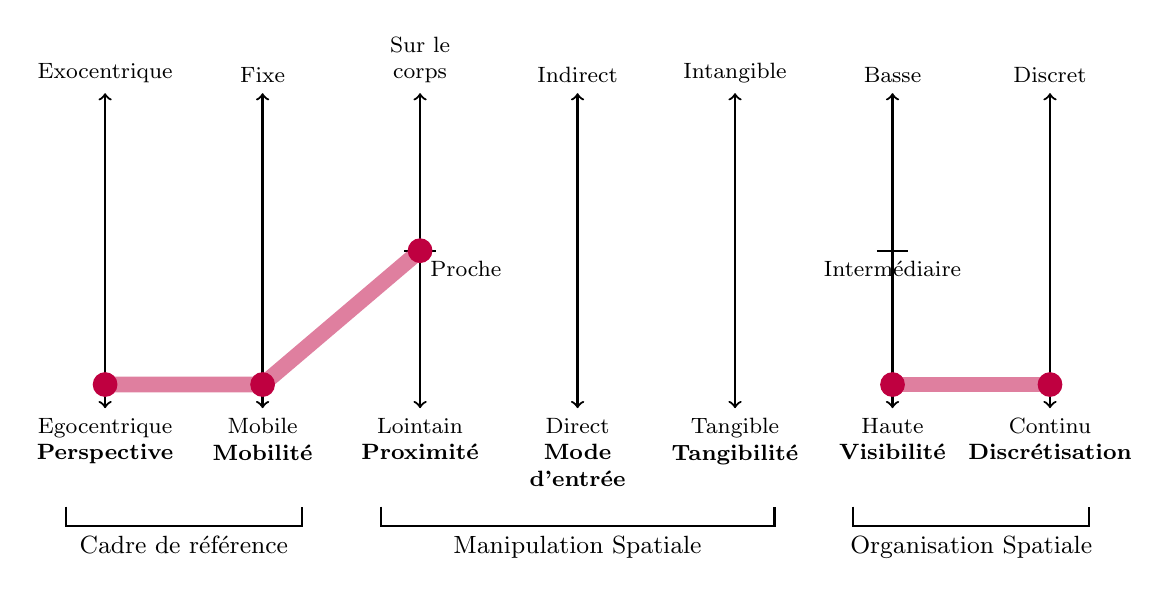
\begin{tikzpicture}[font=\footnotesize] 
    \draw [thick] (-0.5,-1.25) -- (-0.5,-1.5) -- (1,-1.5) node [below] {\small Cadre de référence} -- (2.5,-1.5) -- (2.5,-1.25) ;
    \draw [thick, <->] (0,0) node [below, align=center] {Egocentrique\\\textbf{Perspective}} -- (0,4) node [above] {Exocentrique} ;
    \draw [thick, <->] (2,0) node [below, align=center] {Mobile\\\textbf{Mobilité}} -- (2,4) node [above] {Fixe} ;

    \draw [thick] (3.5,-1.25) -- (3.5,-1.5) -- (6,-1.5) node [below] {\small Manipulation Spatiale} -- (8.5,-1.5) -- (8.5,-1.25) ;
    \draw [thick, <->] (4,0) node [below, align=center] {Lointain\\\textbf{Proximité}} -- (4,4) node [above, align=center] {Sur le\\corps} ;
    \draw [thick] (3.8,2) -- (4,2) node [below right] {Proche} -- (4.2,2) ;
    \draw [thick, <->] (6,0) node [below, align=center] {Direct\\\textbf{Mode}\\\textbf{d'entrée}} -- (6,4) node [above] {Indirect} ;
    \draw [thick, <->] (8,0) node [below, align=center] {Tangible\\\textbf{Tangibilité}} -- (8,4) node [above] {Intangible} ;

    \draw [thick] (9.5,-1.25) -- (9.5,-1.5) -- (11,-1.5) node [below] {\small Organisation Spatiale} -- (12.5,-1.5) -- (12.5,-1.25) ;
    \draw [thick, <->] (10,0) node [below, align=center] {Haute\\\textbf{Visibilité}} -- (10,4) node [above] {Basse} ;
    \draw [thick] (9.8,2) -- (10,2) node [below] {Intermédiaire} -- (10.2,2) ;
    \draw [thick, <->] (12,0) node [below, align=center] {Continu\\\textbf{Discrétisation}} -- (12,4) node [above] {Discret} ;

    \draw [draw=purple, fill=purple] (0,0.3) circle [radius=0.15] ;
    \draw [draw=purple, fill=purple] (2,0.3) circle [radius=0.15] ;
    \draw [draw=purple, fill=purple] (4,2) circle [radius=0.15] ;
    \draw [draw=purple, fill=purple] (10,0.3) circle [radius=0.15] ;
    \draw [draw=purple, fill=purple] (12,0.3) circle [radius=0.15] ;
    \draw [purple, line width=0.2cm, opacity=0.5] (0,0.3) -- (2,0.3) -- (4,2) ;
    \draw [purple, line width=0.2cm, opacity=0.5] (10,0.3) -- (12,0.3);
  \end{tikzpicture}%
}{
  Application du cadre de conception \texten{Ethereal Planes} à notre concept de téléphone à affichage étendu.
}


\section{Applications potentielles}
\label{sec:concept_applications}

Nous distinguons tout d'abord deux modes de vues pour afficher du contenu dans un VESAD :
\begin{itemize}
  \item Vue multi-fenêtres \reffigureETSp{HandheldVESADApp} : une application utilise l'écran physique tandis que de multiples applications sont placées autour dans l'écran virtuel sous forme de fenêtres, comme l'IHM du Personal Cockpit \citep{Ens2014}.
  \item Vue étendue \reffigureETSp{HandheldVESADExtended} : une seule application utilise tout les écrans physique et virtuel comme seul écran étendu, de manière similaire à l'IHM de Multifi \citep{Grubert2015}.
\end{itemize}
\bigskip

En vue multi-fenêtres, idée : l'utilisateur organise son espace, sous forme d'une grille ou librement ?
Par exemple : prises de notes en regardant un cours en ligne avec applications notes + wikipedia + youtube
Multi-tâches comme on peut le faire sur un pc
For example, the phone and VESAD could display multiple phone-sized screen-fulls containing sets of app launcher icons and/or running apps \reffigureETSp{HandheldVESADApps.jpg}

\figureLayoutETS{HandheldVESADApp}{%
  \subfigureETS{HandheldVESADApps.jpg}{Plusieurs applications affichées dans des fenêtres différentes sur l'écran virtuel en parallèle à celle sur l'écran physique.}%
  \figurehspace%
  \subfigureETS{HandheldVESADApps2.jpg}{Wrist : une rotation de la main permet de rapidement changer l'application sur l'écran physique.}%
}{
  Photomontages d'un VESAD en vue multi-fenêtres, où de multiples applications se partagent l'écran étendu.
}

En vue étendue
Focus sur une app, comme on le fait sur un téléphone

The VESAD can show an extended view of content already on the phone. \reffigureETS{HandheldVESADMap.jpg} shows this for a geographic map.

The VESAD can provide information that refers to the content on the phone. The content on the phone might be a user interface or a document, while the VESAD displays tooltips, annotations, or callouts \reffigureETSp{HandheldVESADTooltip.jpg}.

The VESAD could display some content that is controlled with a UI on the phone. For example, the phone might show a gallery of thumbnails, where selecting one thumbnail causes an enlarged photo to be displayed on the VESAD \reffigureETSp{HandheldVESADDogs.jpg}. As another example, the phone might display video and audio player controls, while the VESAD shows the video playback. A third example of this would be a text chat or video conferencing application, where the phone displays a list of contacts and options to invite people to conversations, while the VESAD displays a history of the text messages exchanged and/or videos of participants.
and/or web browser tabs : ressemble à du multi-fenêtres, mais la structure de l'affichage est contrôlé par l'app, pas par l'utilisateur (onglets à gauche et à droite, favoris en haut : gestes un doigt pour l'écran physique, deux pouces pour l'écran étendu : défilement gauche-droite des onglets, haut pour favoris, droit pour supprimer, direct touch sur écran virtuel possible)

The phone and VESAD could also be used for overview + details or focus + context visualizations of data \cite{cockburn2009,burigat2013}. In such cases, either display modality could be used to show extra detail. For example, in \reffigureETSp{HandheldVESADDogs.jpg}, the gallery of thumbnails on the phone serves as a kind of overview, with the VESAD showing a detailed (zoomed in) view of one selected photo. However, these roles could be swapped to allow for more thumbnails to be visible at once (in the VESAD) while also displaying a single photo with greater pixel density (on the phone).

\figureLayoutETS{HandheldVESADExtended}{%
  \subfigureETS{HandheldVESADMap.jpg}{Une carte de navigation.}%
  \figurehspace%
  \subfigureETS{HandheldVESADDogs.jpg}{Une galerie d'images.}%
  \figurehspace%
  \subfigureETS{HandheldVESADTooltip.jpg}{Info-bulles dans l'écran virtuel.}%
}{
  Photomontages d'applications en vue étendue, exploitant tout l'écran étendu du VESAD.
}

L'écran virtuel peut également être utilisé par le système d'exploitation en parallèle de ce que fait l'utilisateur, comme sur un téléphone actuel avec la bare de notifications, ou un PC avec la barre de tâches

The VESAD can display alternative versions of what the phone already displays. \reffigureETS{HandheldVESADApps.jpg} also indicates how the VESAD could display notifications with details (for example, the sender's name and subject of incoming messages,
descriptions of upcoming appointments, and a chart of battery level over time).

Notifications en profondeurs\\
Justification : Robertson1998 - Data mountain. Overlapping windows on a 2D screen adds more cognitive load than arranging a stack of physical papers in  3D space [7]. (Lee, 2013 pour DataMoutain)D\\
Ça fonctionne de s'appuyer sur la mémoire spatiale humaine : justifie notre concept d'organiser l'espace autour du cellulaire comme une idée pertinente. On pourrait organiser les applications dans le plan et en profondeur le long d'un plan qui part de la base du cellulaire avec une pente positive : cela permet de voir toutes les applications, comme sur des gradins d'un stade (c'est ce que Data Moutain suggère comme placement des app dans l'espace)

Copier/coller : zone en bas de l'écran tactile


\section{Techniques d'interactions}
\label{sec:concept_interaction_techniques}

Une de nos questions de recherche \autorefp{sec:research_problem} est quelle technique d'interaction est la plus adaptée pour un téléphone étendu par un VESAD. On peut en effet penser à différentes techniques qui ont été explorées dans la littérature pour interagir dans avec telle IHM :

\begin{itemize}
  \item Pointer directement le contenu avec une main virtuelle, utilisé par le Personal Cockpit \cite{Ens2014} et exploré par \cite{Piumsomboon2013}.
  \item Utiliser l'écran tactile du téléphone, comme dans la condition \condition{Smartwatch referenced} de MultiFi \citep{Grubert2015} ou dans une application ARCore ou ARKit.
  \item Utiliser un pointeur virtuel et des gestes de sélection \cite{Wilson2006}, comme sur un Microsoft HoloLens.
  \item Via des commandes vocales, évaluées par \cite{Piumsomboon2014}.
\end{itemize}
\bigskip

\figureETS{HandheldVESADSlideToHang.jpg}{
  Un geste Slide to Hang permet à un utilisateur de détacher une application de l'écran étendu pour la fixer en l'air, contre une surface ou relativement à son corps. Dans ce photomontage, un utilisateur détache dans un premier temps une page web en l'air, puis un lecteur vidéo.
}

En outre, nous présentons deux nouvelles techniques d'interactions pour notre IHM :
\begin{enumerate}
  \item Wrist : un mouvement de la main tenant le téléphone permet de changer rapidement l'affichage sur l'écran physique. La \reffigureETS{HandheldVESADApps2.jpg} montre par exemple l'utilisateur tournant son téléphone à \ang{90} environ vers la droite pour changer l'application affichée sur l'écran physique. Un pointeur virtuel suivant le regard ou la tête de l'utilisateur permettrait de choisir l'application sur l'ecran virtuel à utiliser, par exemple parmi une liste d'icônes d'applications.
  \item Slide to Hang : un geste de glissement permet de détacher une fenêtre de l'écran étendu et la fixer en l'air. La \reffigureETS{HandheldVESADSlideToHang.jpg} montre l'utilisateur faisant un geste de glissement (\texten{slide} en anglais) sur le téléphone pour fixer en l'air la fenêtre qui y est affichée. La fenêtre peut être alors placée à un endroit fixe sur un mur ou en l'air, comme avec le Microsoft HoloLens, ou relativement à son propre corps, comme dans le Personal Cockpit \cite{Ens2014}. Ce geste de glissement peut se faire avec deux doigts simultanément sur le téléphone pour distinguer d'actions faites sur l'application, ou avec la main entière dans l'écran virtuel. Un geste de la fenêtre fixée vers l'écran étendu permettrait de la ramener relative au téléphone.
\end{enumerate}